\documentclass[12pt]{article}
\usepackage{graphicx}
\usepackage{float}
\usepackage{amsmath}
\title{Experiment 10: Tone Generator}
\author{Annirudh K P\\%
210070009}
\date{October 22, 2022}
\begin{document}

\maketitle

\section{Overview of the experiment}
\paragraph{}
In this experiment, we worked on some sequential circuit designs using behavioural modelling on VHDL. The problem statement of this experiment is to design a Tone Generator using the already acquired knowledge of Clock Divider from the previous lab. The objective of this experiment is to understand the Quartus Design Flow, work with the Xen10 Board, use Pin Planning, and give us hands on experience over different technical glitches/problems we may face in this piece of software which has been made unwantedly hard.

\section{Experimental Set-up}

\subsection{Design Schematics}
The idea behind the design of Clock divider, which is to be used for he tone generator is as shown:

\begin{figure}[H]
\centering
  \includegraphics*[scale=0.7]{Images/ClockDiv_Design.jpeg}
\end{figure}

Further the set of frequencies and counts used for the tone generator are as follows:

\begin{figure}[H]
\centering
  \includegraphics*[scale=0.5]{Images/ToneGen_Design.jpeg}
\end{figure}

\subsection{Description of Components}
\subsubsection{Clock Divider}
\begin{verbatim}
library ieee;
use ieee.std_logic_1164.all;
use ieee.numeric_std.all;

entity tone_generator is
port (clk_50 : in std_logic;
		switch : in std_logic_vector(7 downto 0);
		LED_out : out std_logic_vector(7 downto 0);
		final_out : out std_logic);
end entity tone_generator;

architecture bhv of tone_generator is
signal count0, count1, count2, count3, count4, count5, 
count6, count7 : integer := 1;
signal clk_out_temp : std_logic_vector(7 downto 0) := "00000000";

begin
clock_proc:process(clk_50)
begin
	if(clk_50='1' and clk_50' event) then
		count0 <= count0 + 1;
		count1 <= count1 + 1;
		count2 <= count2 + 1;
		count3 <= count3 + 1;
		count4 <= count4 + 1;
		count5 <= count5 + 1;
		count6 <= count6 + 1;
		count7 <= count7 + 1;
	
		if (count0 = 104168) then
			count0 <= 1;
			clk_out_temp(0) <= not clk_out_temp(0);
		end if;
		if (count1 = 92584) then
			count1 <= 1;
			clk_out_temp(1) <= not clk_out_temp(1);
		end if;
		if (count2 = 83333) then
			count2 <= 1;
			clk_out_temp(2) <= not clk_out_temp(2);
		end if;
		if (count3 = 78125) then
			count3 <= 1;
			clk_out_temp(3) <= not clk_out_temp(3);
		end if;
		if (count4 = 69444) then
			count4 <= 1;
			clk_out_temp(4) <= not clk_out_temp(4);
		end if;
		if (count5 = 62500) then
			count5 <= 1;
			clk_out_temp(5) <= not clk_out_temp(5);
		end if;
		if (count6 = 55554) then
			count6 <= 1;
			clk_out_temp(6) <= not clk_out_temp(6);
		end if;
		if (count7 = 52084) then
			count7 <= 1;
			clk_out_temp(7) <= not clk_out_temp(7);
		end if;
	end if;
	
	LED_out <= "00000000";
	if ((switch(0) and (not switch(1)) and (not switch(2)) and (not switch(3)) and 
	(not switch(4)) and (not switch(5)) and (not switch(6)) and (not switch(7))) = '1') then
		LED_out <= "00000000";
		LED_out(0) <= '1';
		final_out <= clk_out_temp(0);
	elsif ((switch(0) and (switch(1)) and (not switch(2)) and (not switch(3)) and
	 (not switch(4)) and (not switch(5)) and (not switch(6)) and (not switch(7))) = '1') then
		final_out <= clk_out_temp(1);
		LED_out <= "00000000";
		LED_out(1) <= '1';
	elsif ((switch(0) and (switch(1)) and (switch(2)) and (not switch(3)) and (not switch(4)) 
	and (not switch(5)) and (not switch(6)) and (not switch(7))) = '1') then
		final_out <= clk_out_temp(2);
		LED_out <= "00000000";
		LED_out(2) <= '1';
	elsif ((switch(0) and (switch(1)) and (switch(2)) and (switch(3)) and (not switch(4))
	and (not switch(5)) and (not switch(6)) and (not switch(7))) = '1') then
		final_out <= clk_out_temp(3);
		LED_out <= "00000000";
		LED_out(3) <= '1';
	elsif ((switch(0) and (switch(1)) and (switch(2)) and (switch(3)) and (switch(4)) 
	and (not switch(5)) and (not switch(6)) and (not switch(7))) = '1') then
		final_out <= clk_out_temp(4);
		LED_out <= "00000000";
		LED_out(4) <= '1';
	elsif ((switch(0) and (switch(1)) and (switch(2)) and (switch(3)) and (switch(4)) 
	and (switch(5)) and (not switch(6)) and (not switch(7))) = '1') then
		final_out <= clk_out_temp(5);
		LED_out <= "00000000";
		LED_out(5) <= '1';
	elsif ((switch(0) and (switch(1)) and (switch(2)) and (switch(3)) and (switch(4)) 
	and (switch(5)) and (switch(6)) and (not switch(7))) = '1') then
		final_out <= clk_out_temp(6);
		LED_out <= "00000000";
		LED_out(6) <= '1';
	elsif ((switch(0) and (switch(1)) and (switch(2)) and (switch(3)) and (switch(4)) 
	and (switch(5)) and (switch(6)) and (switch(7))) = '1') then
		final_out <= clk_out_temp(7);
		LED_out <= "00000000";
		LED_out(7) <= '1';
	else 
		final_out <= '0';
		LED_out <= "00000000";
	end if;
	
end process;
end bhv;
\end{verbatim}

\section{Observations}
 
The code after appropriate pin planning, (in form of .svf file) was flashed onto the Xen10 board. Then like a keyboard, the LEDs are planned to blink when the respective key is played. The Header 1 Pin 1 is planned to give the output frequency according to the switch configuration. Using transistor, breadboard and a speaker, the circuit was set up. The output was verified, which also verified the working of the logic for the Tone Generator.

\begin{figure}[H]
\centering
  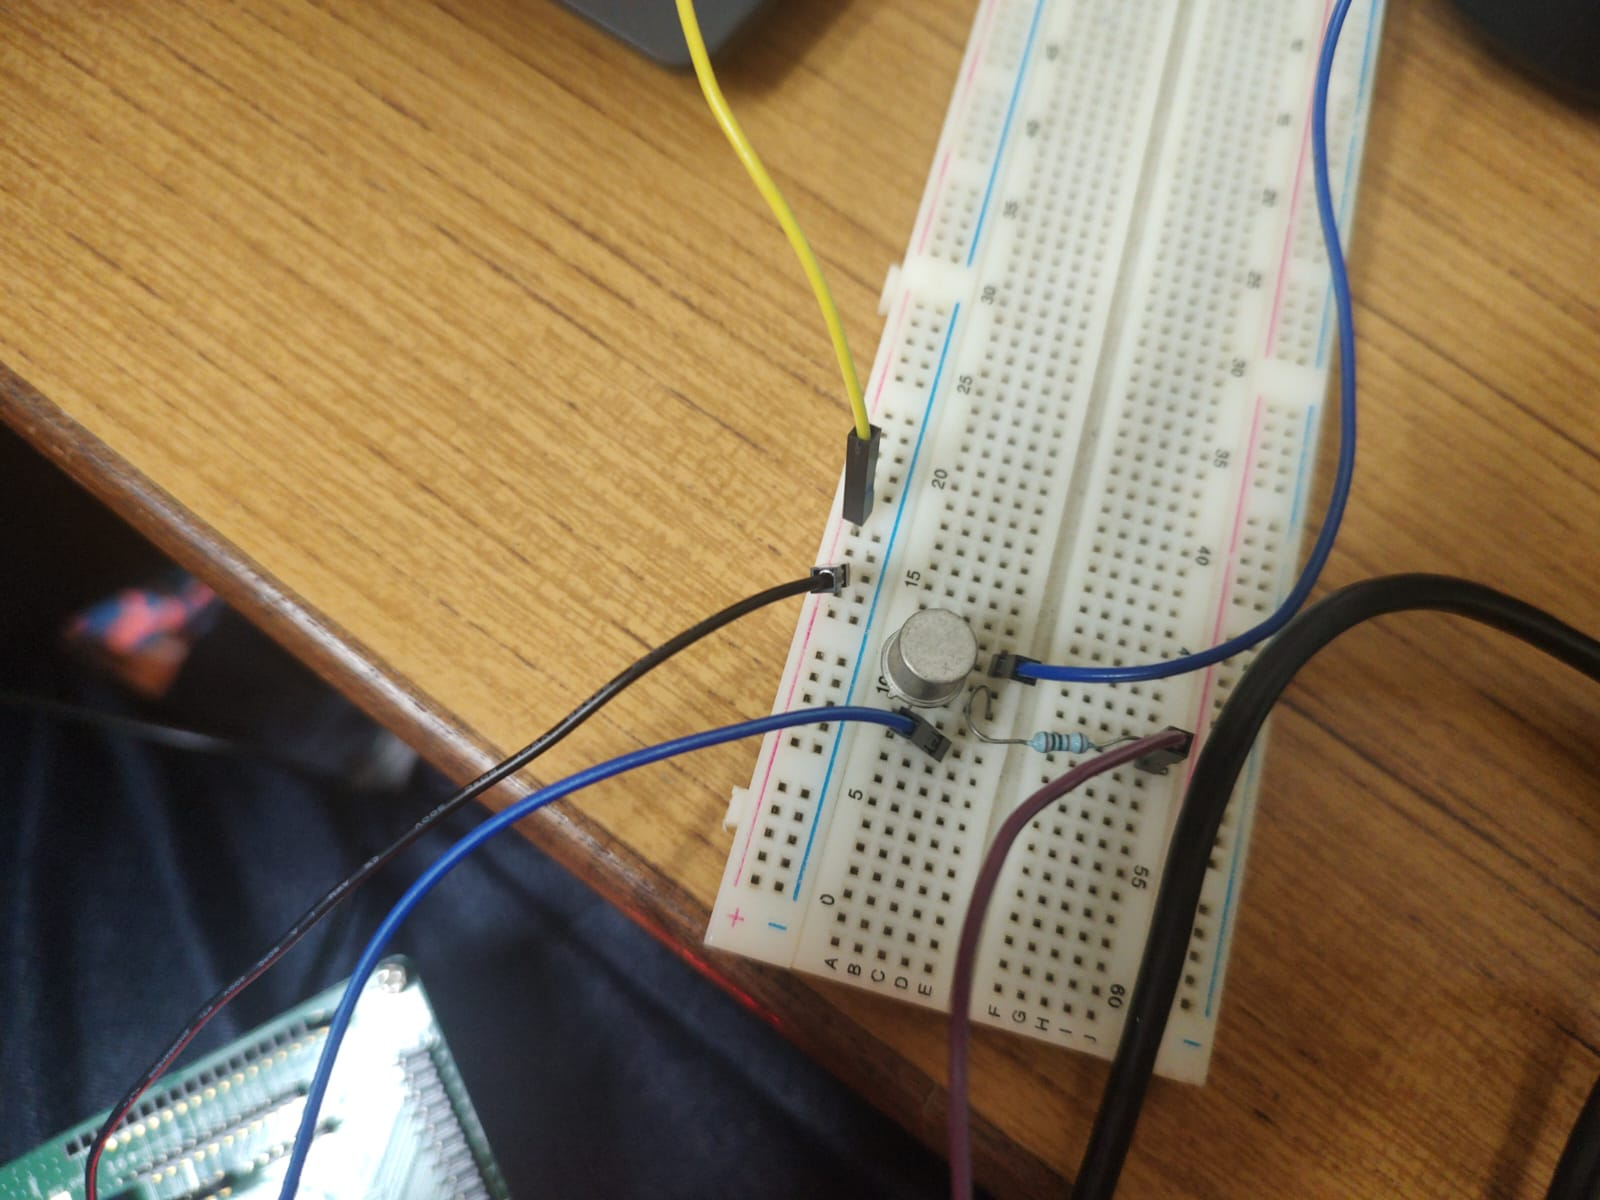
\includegraphics[scale=0.2]{Images/ToneGen_Circuit1.jpg}
  \caption{Tone Generator Circuit 1}
\end{figure}

\begin{figure}[H]
\centering
  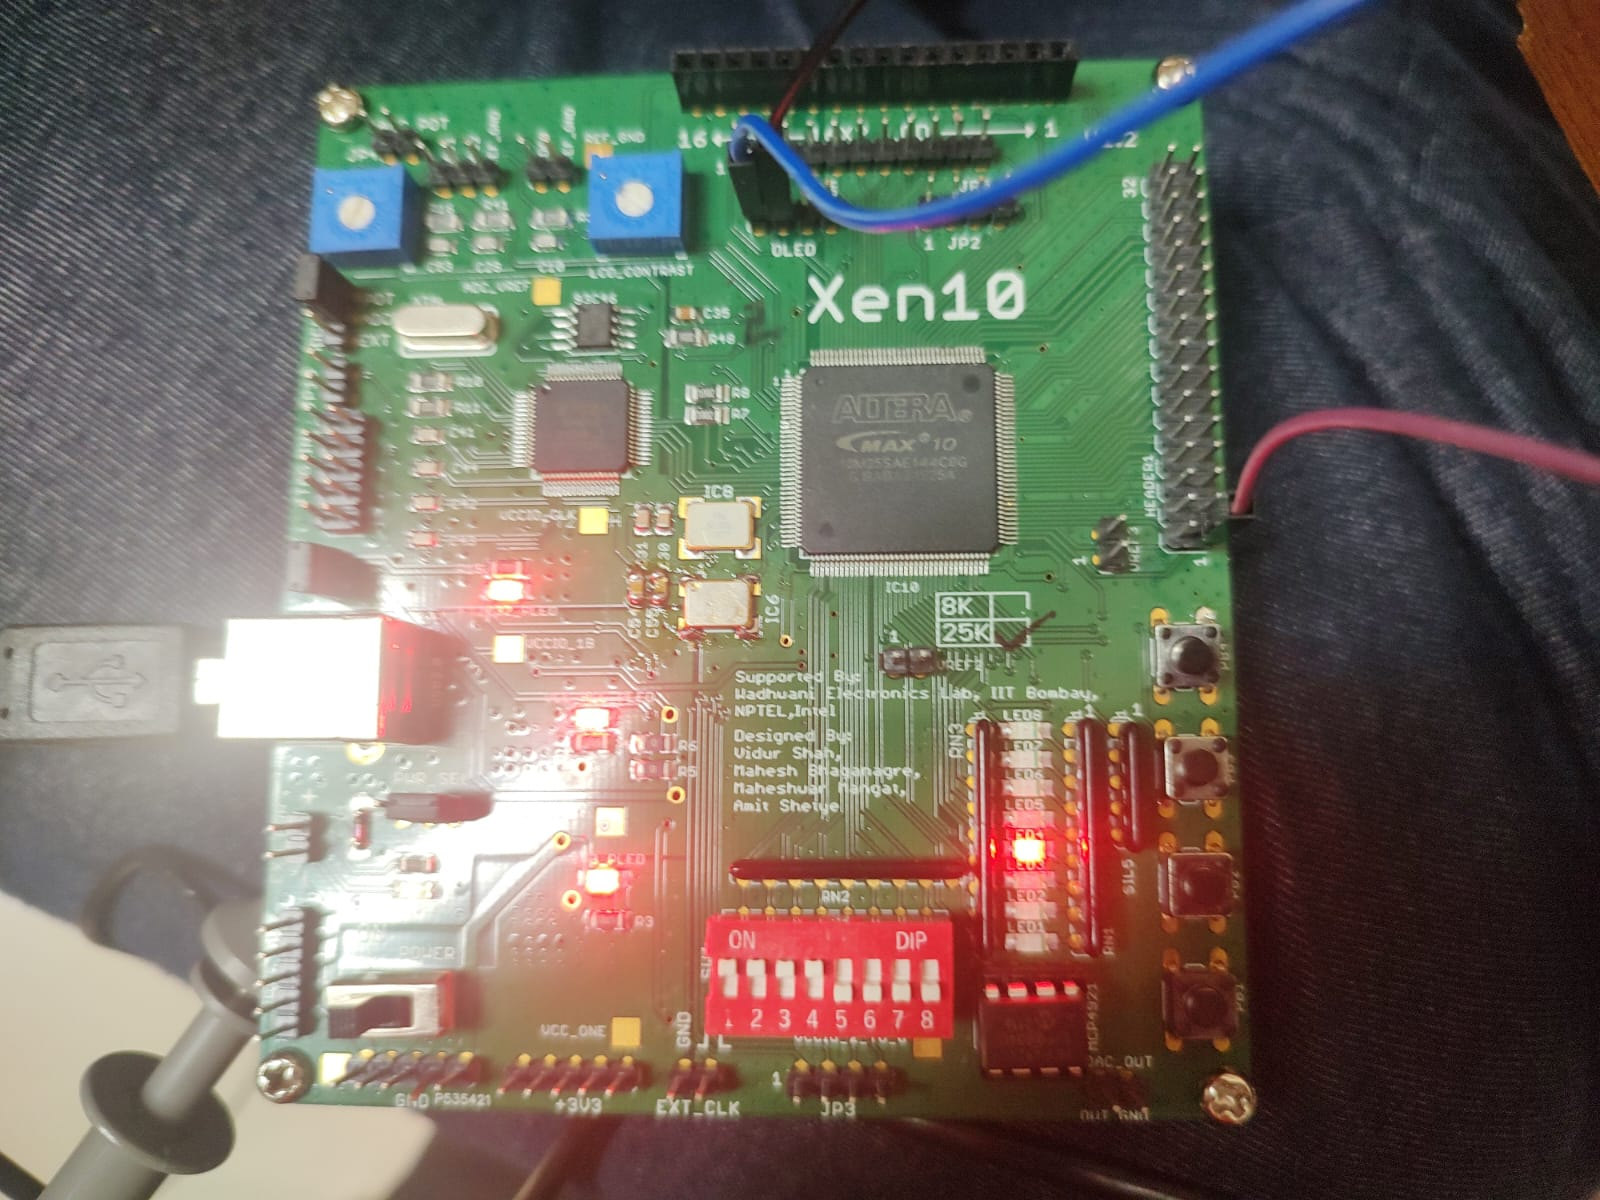
\includegraphics[scale=0.2]{Images/ToneGen_Circuit2.jpg}
  \caption{Tone Generator Circuit 2}
\end{figure}

\begin{figure}[H]
\centering
  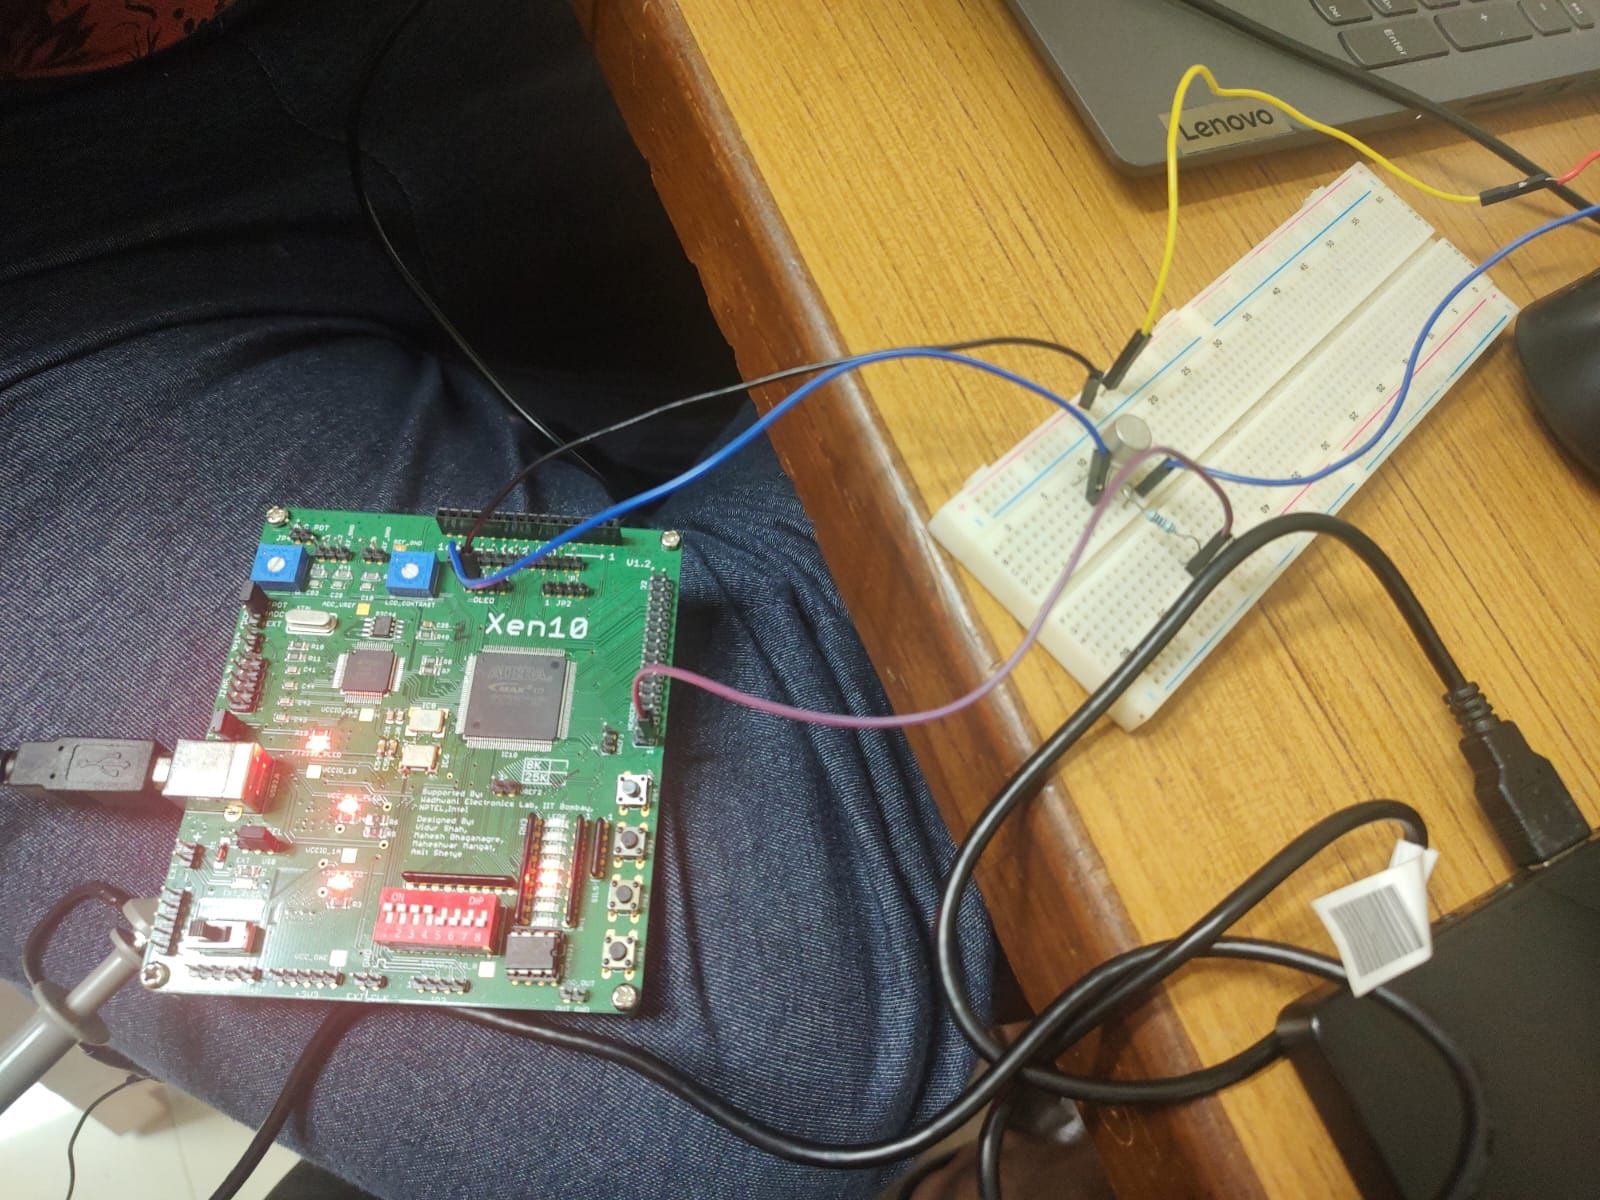
\includegraphics[scale=0.2]{Images/ToneGen_Circuit3.jpg}
  \caption{Tone Generator Circuit 3}
\end{figure}

\end{document}